% Settings for the default beamer theme
\documentclass[english, aspectratio=169]{beamer}
\usepackage[T1]{fontenc}
\usepackage[utf8]{inputenc}
\usepackage{tabularx}
\usepackage{babel}
\usepackage[ruled,vlined]{algorithm2e}
\SetAlgorithmName{Algoritmus}{algoritmus}{List of Algorithms}
\setcounter{secnumdepth}{3}
\setcounter{tocdepth}{3}

\makeatletter

\newcommand\makebeamertitle{\frame{\maketitle}}

% (ERT) argument for the TOC
\AtBeginDocument{%
  \let\origtableofcontents=\tableofcontents
  \def\tableofcontents{\@ifnextchar[{\origtableofcontents}{\gobbletableofcontents}}
  \def\gobbletableofcontents#1{\origtableofcontents}
}

% Theme settings
\usetheme{Frankfurt}
\usecolortheme{default}
\usefonttheme[onlymath]{serif}

% Template settings
\setbeamertemplate{navigation symbols}{}
\setbeamertemplate{blocks}[rounded][shadow=false]
\setbeamertemplate{title page}[default][colsep=-4bp, rounded=true, shadow=false]
\makeatother

% Define a custom darker red color
\definecolor{DarkerRed}{RGB}{139,0,0} % Adjust the RGB values as needed

% Use the newly defined color in Beamer theme elements
\setbeamercolor{structure}{fg=DarkerRed} % Changes basic structural elements to Darker Red
\setbeamercolor{title in head/foot}{bg=DarkerRed} % Changes the title in header/footer to Darker Red


\begin{document}

% Title page
\section{Neurális hálók felépítése}
\title[]{Üzleti Elemzések Módszertana}
\subtitle{10. Előadás: Neurális hálózatok}
\author[Kuknyó Dániel]{Kuknyó Dániel\\Budapesti Gazdasági Egyetem}
\date{2023/24\\2.félév}
\makebeamertitle

% Table of contents slide
\begin{frame}
\tableofcontents{}
\end{frame}

% Table of contents of the current section
\begin{frame}
\tableofcontents[currentsection]
\end{frame}

\begin{frame}{A biológiai neurontól a mesterségesig}
\begin{columns}
\begin{column}{.5\textwidth}
A madarak repülésre inspirálták az embert, a bogáncsok a tépőzárat ihlették. A logikus lépés az volt, hogy az agy által inspirálódva megpróbál az ember gépeket létrehozni.
\begin{center}
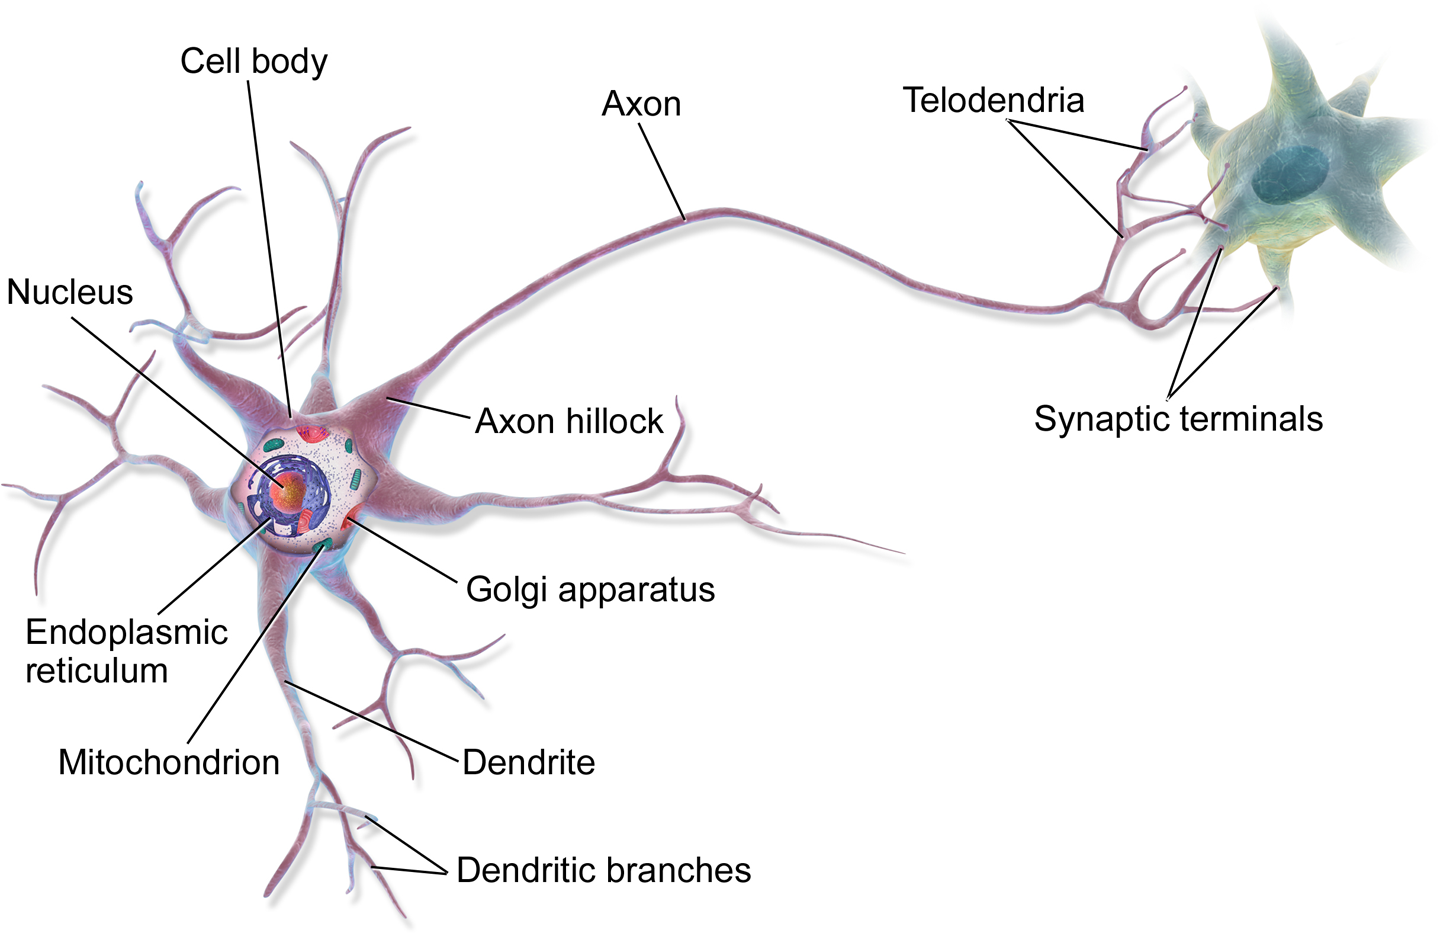
\includegraphics[width=6cm, height=7cm, keepaspectratio]{images/neural_1.png}
\end{center}
\end{column}
\begin{column}{.5\textwidth}
Ahogy repülők sem csapkodnak a szárnyaikkal, a mesterséges neuronok is meglehetősen különböznek a biológiai unokatestvéreiktől.
\begin{center}
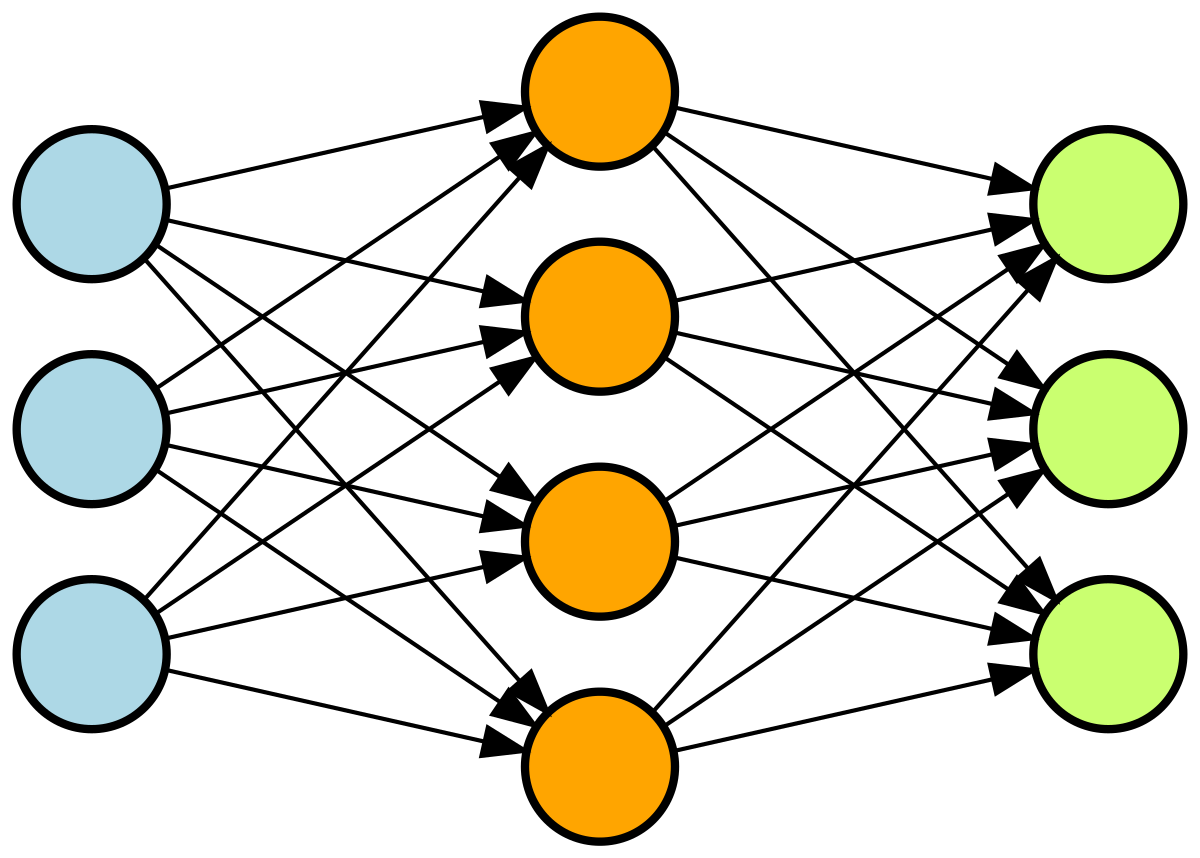
\includegraphics[width=6cm, keepaspectratio]{graphs/neural_1.png}
\end{center}
\end{column}
\end{columns}
\end{frame}

\begin{frame}{Logikai számítások neuronokkal}
\begin{columns}
\begin{column}{.5\textwidth}
Warren McCulloh és Walter Pitts modellezték először a biológiai neuront, ami később a mesterséges neuronként vált ismertté. Egy bináris kimenete, és több bináris bemenete van.\par\smallskip
\textbf{A mesterséges neuron akkor aktiválja az outputját, ha az inputjai meghatározott számban aktiválódnak.}\par\smallskip
Bármilyen összetett logikai kifejezés kifejezhető ilyen neuronokkal: a példában az identitás, és, vagy, xvagy kifejezések konfigurációi láthatók.
\end{column}
\begin{column}{.5\textwidth}
\begin{center}
\only<1>{\[
B = A
\]}
\only<2>{\[
C = A \land B
\]}
\only<3>{\[
C = A \lor B
\]}
\only<4>{\[
C = A \land \lnot B
\]}
\includegraphics<1>[width=5cm, height=5cm, keepaspectratio]{graphs/neural_2.png}
\includegraphics<2>[width=5cm, height=5cm, keepaspectratio]{graphs/neural_3.png}
\includegraphics<3>[width=5cm, height=5cm, keepaspectratio]{graphs/neural_4.png}
\includegraphics<4>[width=5cm, height=5cm, keepaspectratio]{graphs/neural_5.png}
\end{center}
\end{column}
\end{columns}
\end{frame}

\section{Architektúra}

\begin{frame}
\tableofcontents[currentsection]
\end{frame}

\begin{frame}{A perceptron}
\begin{columns}
\begin{column}{.5\textwidth}
Az egyik legegyszerűbb neurális modell a \textbf{perceptron}. Alapja a \textbf{küszöblogikai egység}. Inputjai és outputja valós számok.\par\smallskip
A perceptron minden $x_i$ inputjához egy $w_i$ súly tartozik.\par\smallskip
Első lépésben a modell kiszámolja inputjainak súlyozott szorzatösszegét:
\begin{block}{}
\vspace{-.6cm}
\[
z = w_1x_1 + w_2x_2 + \ldots + w_nx_n = X^TW
\]
\end{block}
Majd ezt az eredményt behelyettesíti egy aktivációs függvénybe:
\begin{block}{}
\vspace{-.2cm}
\[
h_w\left( x \right) = \varphi\left( z \right)
\]
\end{block}
\end{column}
\begin{column}{.5\textwidth}
\begin{center}
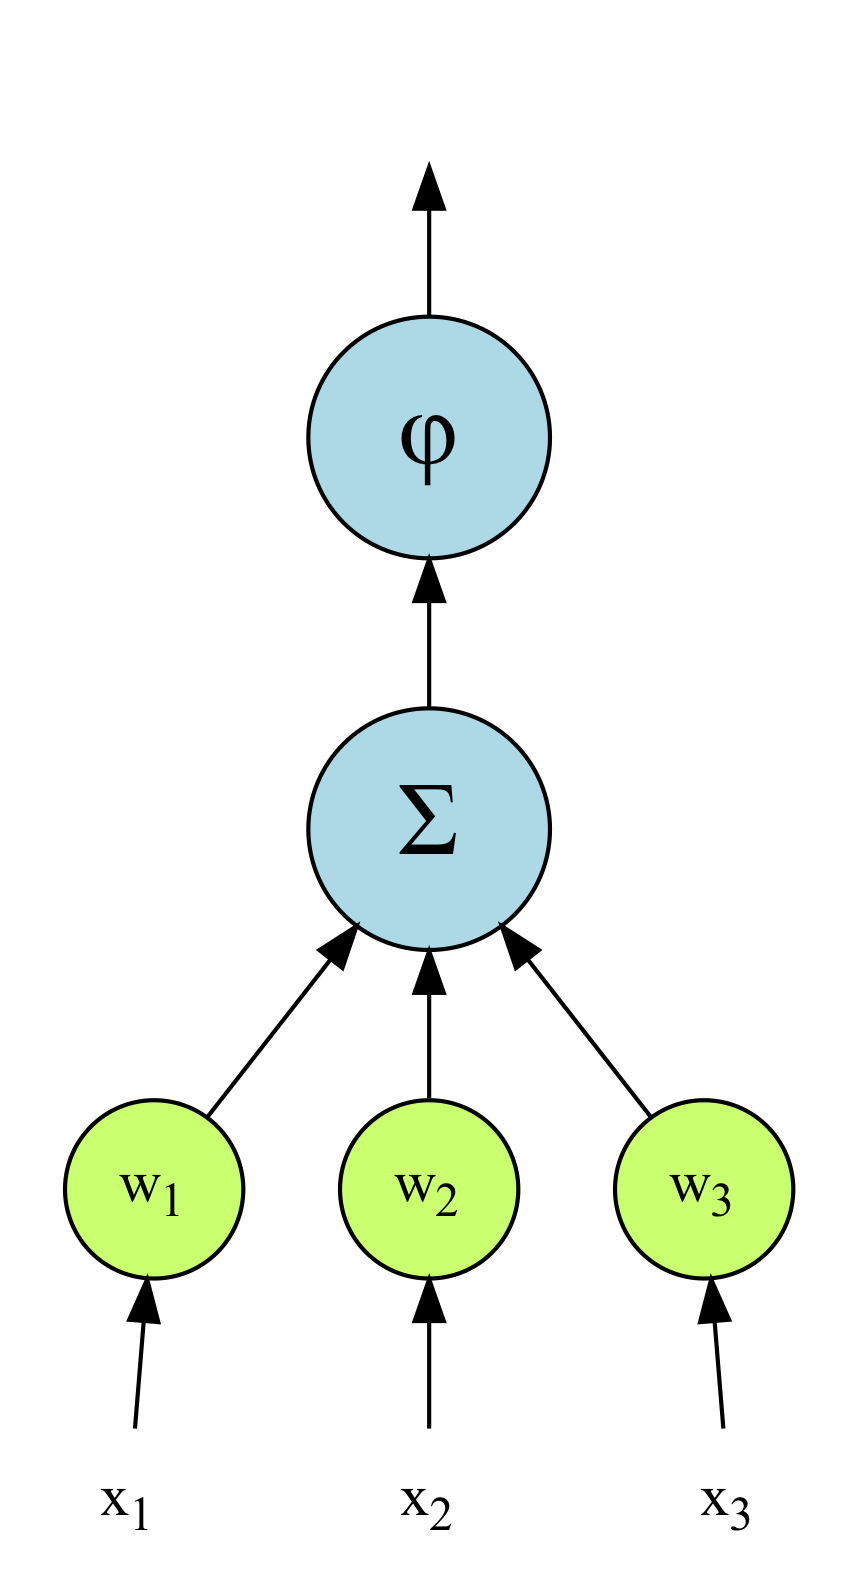
\includegraphics[width=7cm, height=7cm, keepaspectratio]{graphs/neural_6.png}
\end{center}
\end{column}
\end{columns}
\end{frame}

\begin{frame}{Gyakori aktivációs függvények}
\begin{columns}
\begin{column}{.5\textwidth}
\only<1>{A neuron által kiszámolt súlyozott szorzatösszeg egy aktivációs függvénybe kerül behelyettesítésre. \par\smallskip
A neurális hálózatok az aktivációs függvények segítségével \textbf{sajátítanak el komplex mintázatokat}. Az aktivációs függvény vezeti be a neurális hálózatokba a \textbf{nemlineáris transzformációt}, enélkül csak egy lineáris transzformáció lenne.\par\smallskip
A különböző alkalmazásokra külön aktivációs függvények használatosak.}
\only<2>{
\\
$
Sigmoid(x) = \frac{1}{1 + e^x} 
$\\
\vspace{0.5cm}
$
ReLU(x) = max(0, x)
$\\
\vspace{0.5cm}
$
ELU(x)=\begin{cases}_{\alpha(e^{x}-1)}^{x} & _{ha\:x<0}^{ha\:x\geq0}\end{cases}
$\\
\vspace{0.5cm}
$
tanh(x) = \frac{e^{2x} - 1}{e^{2x} + 1}
$\\
\vspace{0.5cm}
$
Leaky\:ReLU(x)=\begin{cases}
_{\alpha\cdot x}^{x} & _{ha\:x<0}^{ha\:x\geq0}\end{cases}
$\\
\vspace{0.5cm}
$
Swish(x,\beta) = \frac{x}{1 + e^{-\beta \cdot x}}
$\\
}
\end{column}
\begin{column}{.5\textwidth}
\begin{center}
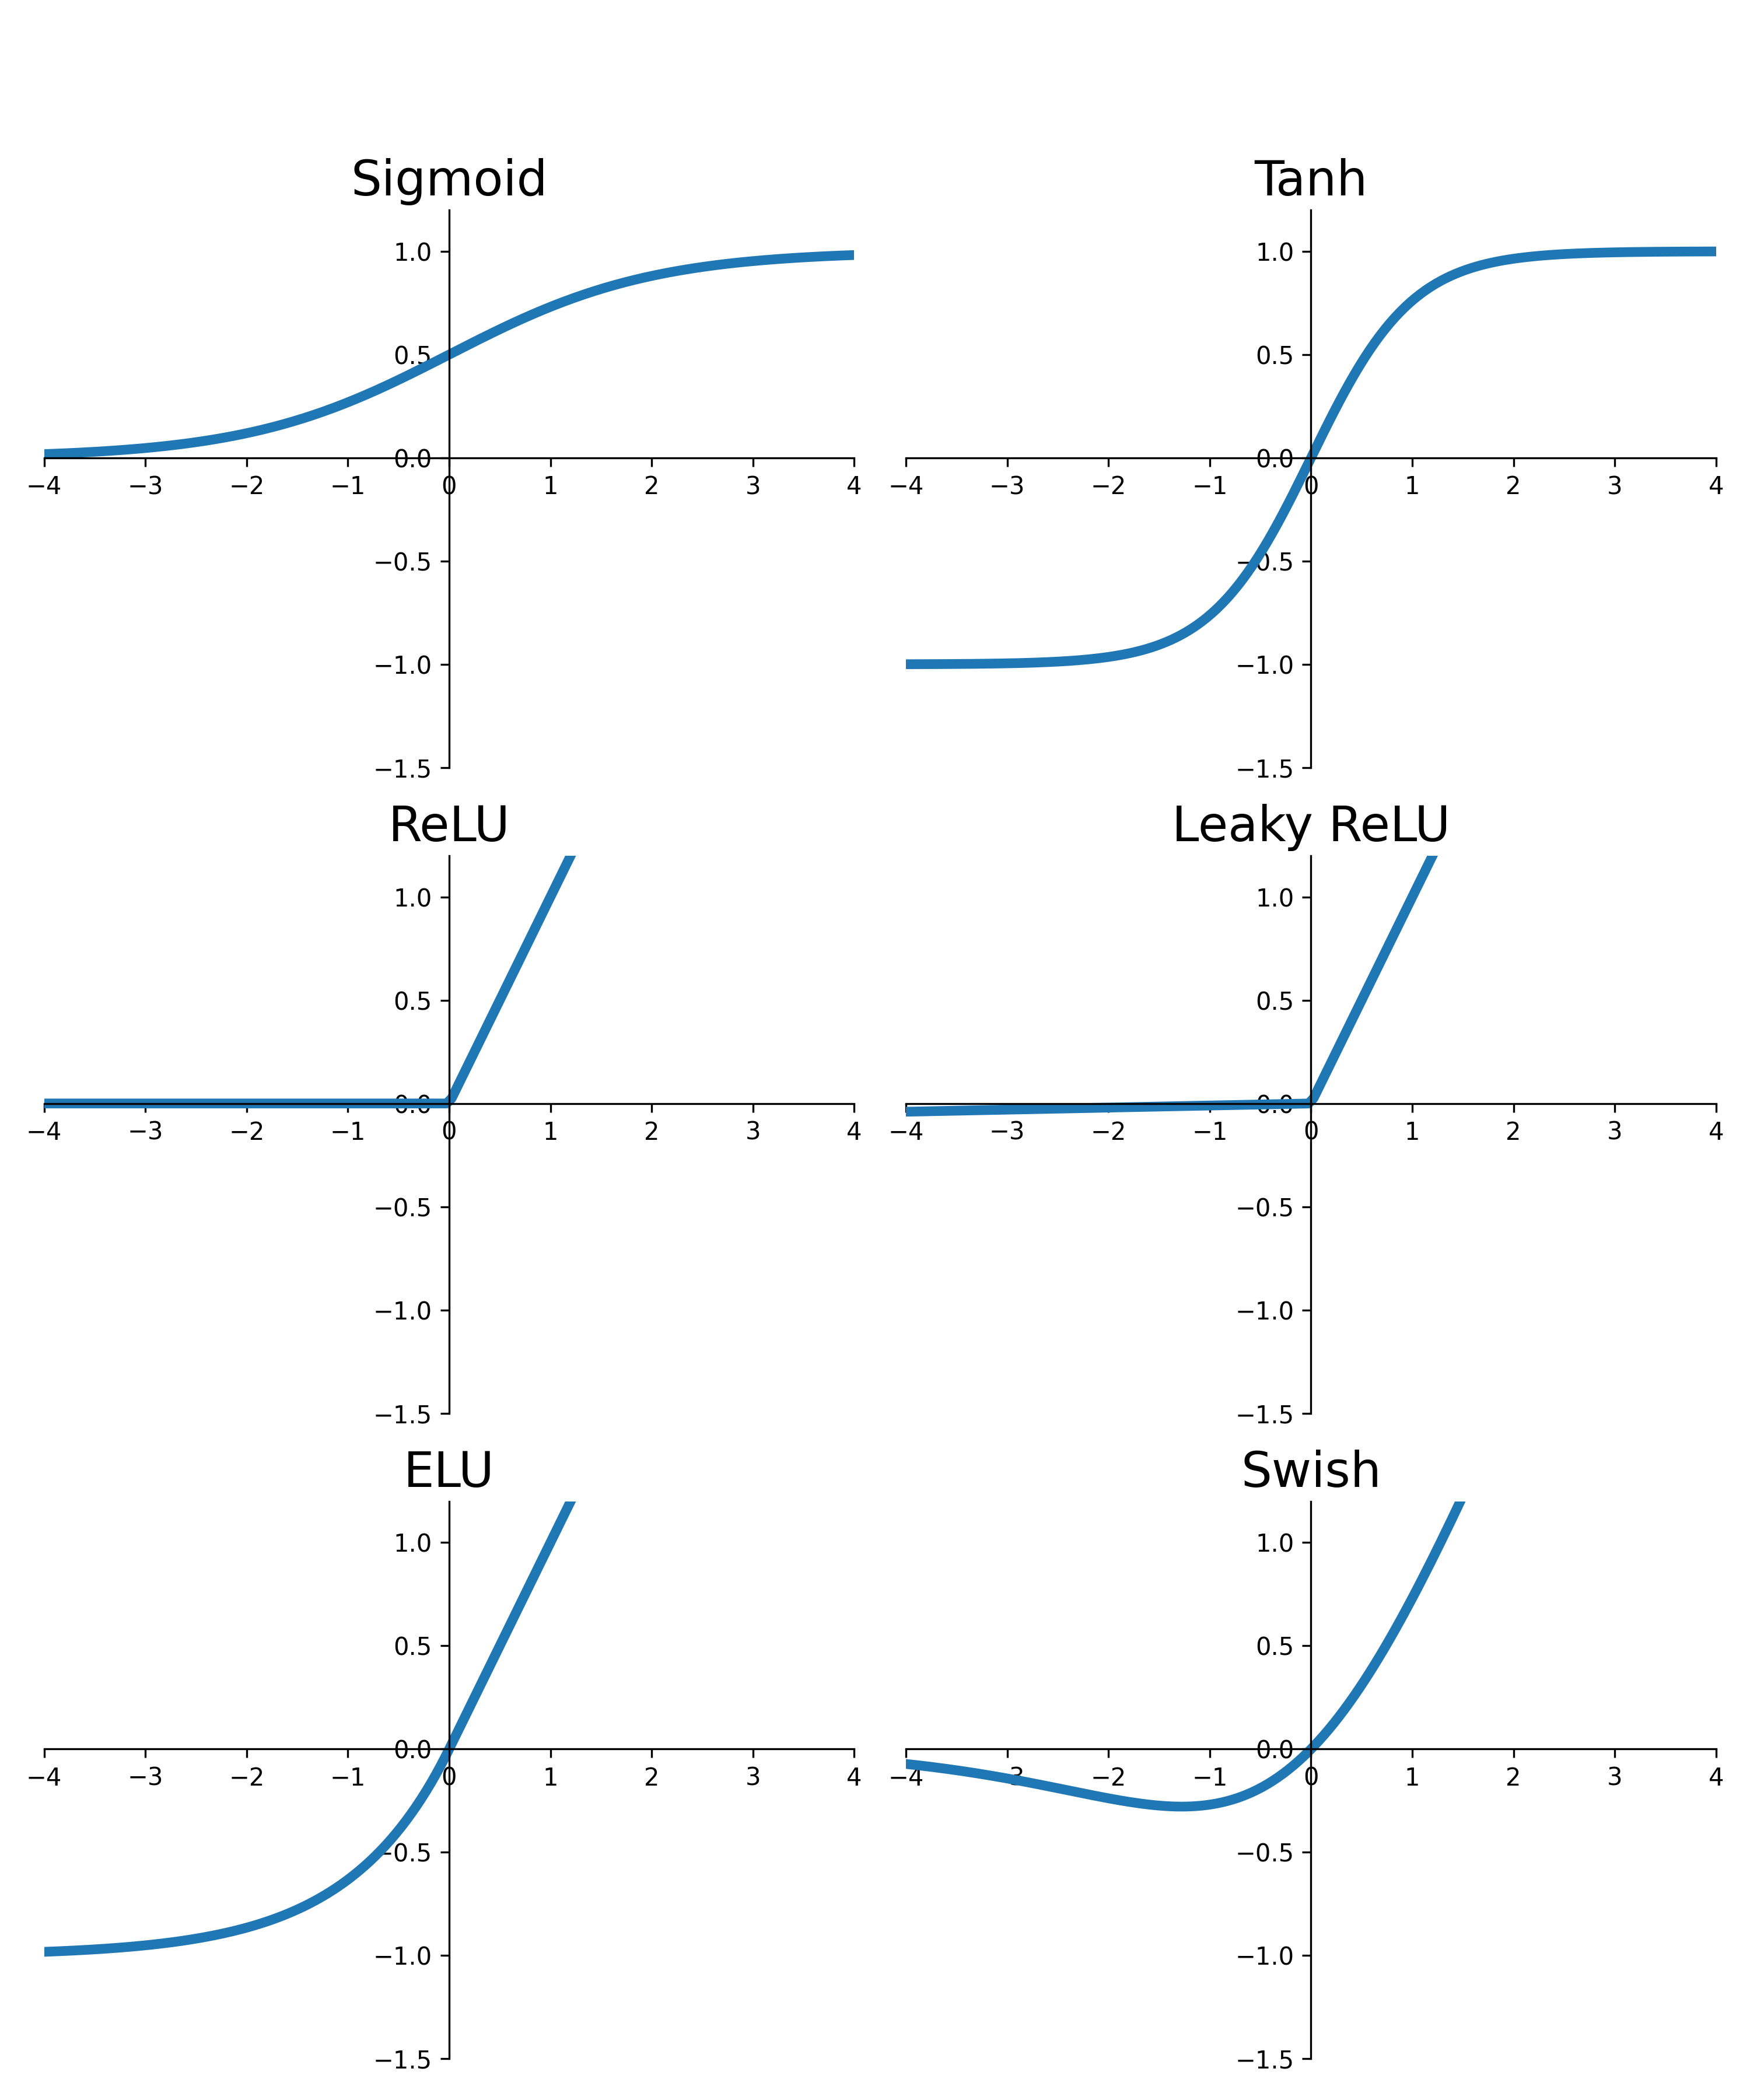
\includegraphics[height=7cm, keepaspectratio]{images/neural_2.png}
\end{center}
\end{column}
\end{columns}
\end{frame}

\begin{frame}{Többrétegű perceptron}
\begin{columns}
\begin{column}{.5\textwidth}
\only<1>{
A többrétegű perceptron esetén a neuronok rétegekbe szerveződötten működnek. Az információ a bemeneti réteg felől a kimeneti réteg irányába áramlik.\par\medskip
\textbf{A legelső réteg neuronjai az adathalmaz jellemzőivel állnak kapcsolatban. Minden további réteg kapcsolata pedig az előző réteg kapcsolataival}.}
\only<2>{
\begin{block}{Teljesen becsatolt réteg kimenete}
\[
h_{w,b}\left( X \right) = \varphi\left( XW + b \right)
\]
Ahol:
\begin{itemize}
	\item $X$: Tanító adathalmaz mátrixa
	\item $W$: A súlyok mátrixa
	\item $b$: Az eltolásokat tartalmazó vektor
	\item $\varphi$: Az aktivációs függvény
\end{itemize}
\end{block}}
\end{column}
\begin{column}{.5\textwidth}
\begin{center}
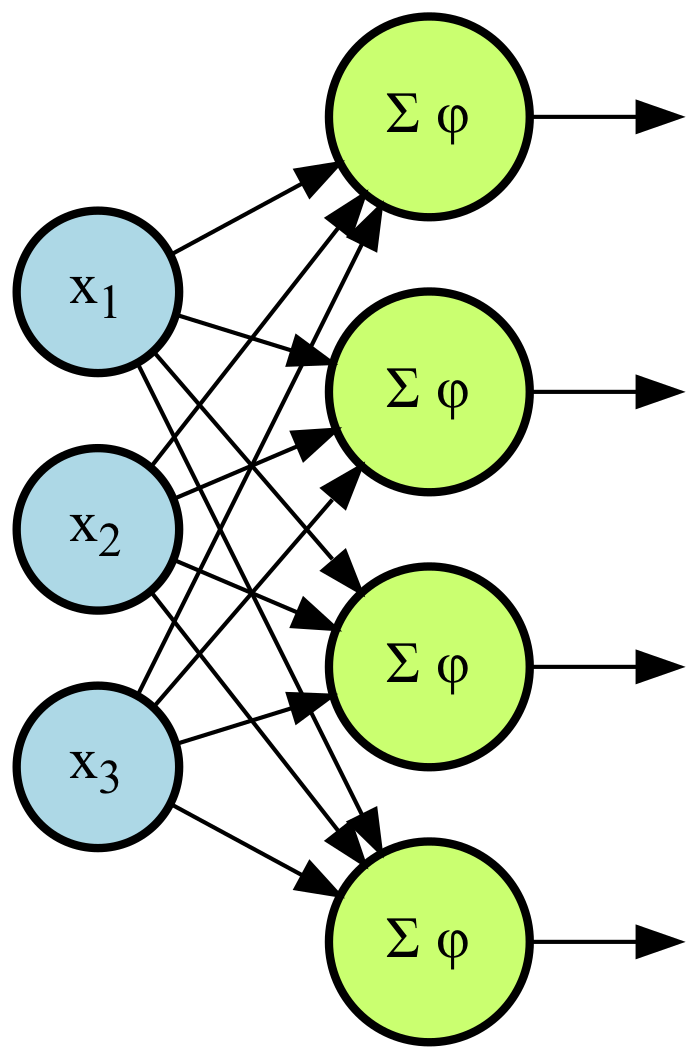
\includegraphics[width=5cm, height=6cm, keepaspectratio]{graphs/neural_7.png}
\end{center}
\end{column}
\end{columns}
\end{frame}

\begin{frame}{Regressziós architektúra}
\begin{columns}
\begin{column}{.5\textwidth}
A többrétegű hálózat egy input réteget, tetszőleges számú rejtett réteget és egy output réteget tartalmaz.\par\medskip
Regressziós problémák esetén az output rétegben \textbf{egy output neuron található, és a predikció a neuron output értéke}. 
\end{column}
\begin{column}{.5\textwidth}
\begin{center}
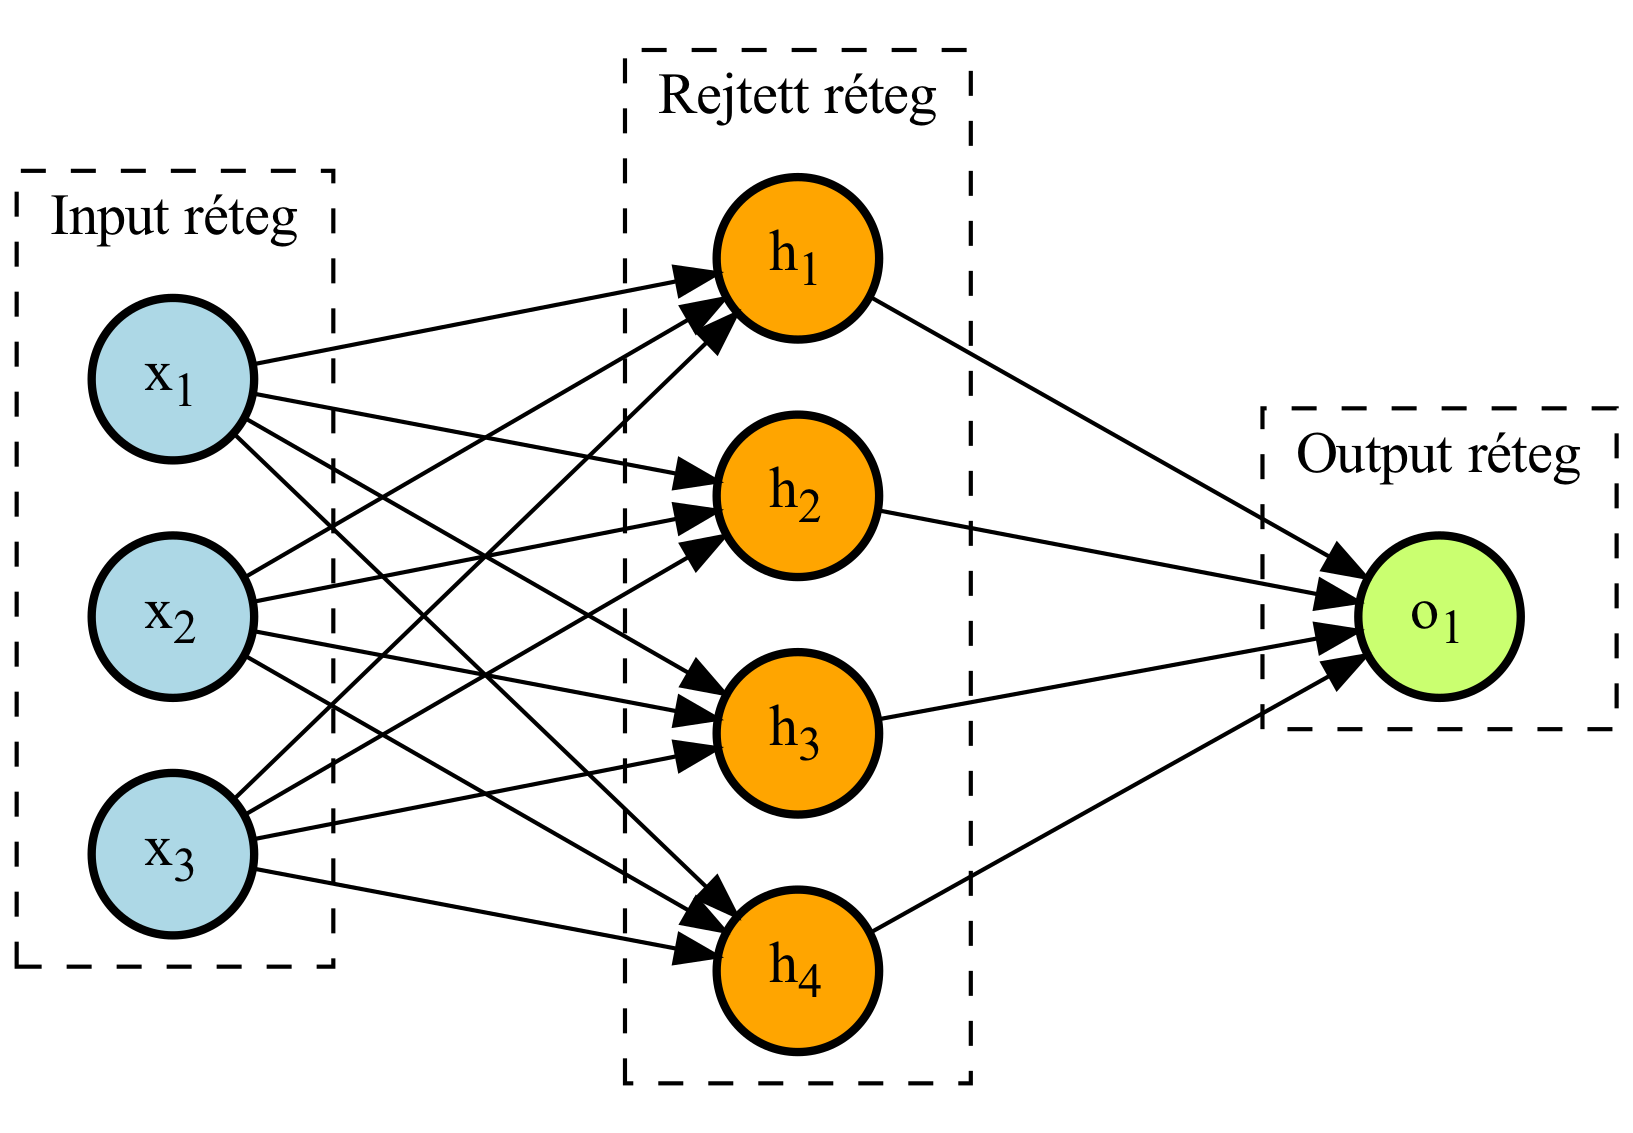
\includegraphics[width=7cm, height=7cm, keepaspectratio]{graphs/neural_8.png}
\end{center}
\end{column}
\end{columns}
\end{frame}

\begin{frame}{Osztályozó architektúra}
\begin{columns}
\begin{column}{.5\textwidth}
Osztályozás esetén a kimeneti rétegbe annyi neuron kerül, ahány lehetséges osztálya van az adatoknak.\par\smallskip
\textbf{Ebben az esetben a neuronok azt becsülik meg, hogy az adott mintaegyed mekkora valószínűséggel tartozik az adott neuronhoz tartozó osztályba}. Ezáltal egy multinomiális valószínűségeloszlás áll elő a kimeneti rétegben.\par\smallskip
Az osztályozó réteg aktivációs függvénye a \textbf{softmax}.
\end{column}
\begin{column}{.5\textwidth}
\begin{center}
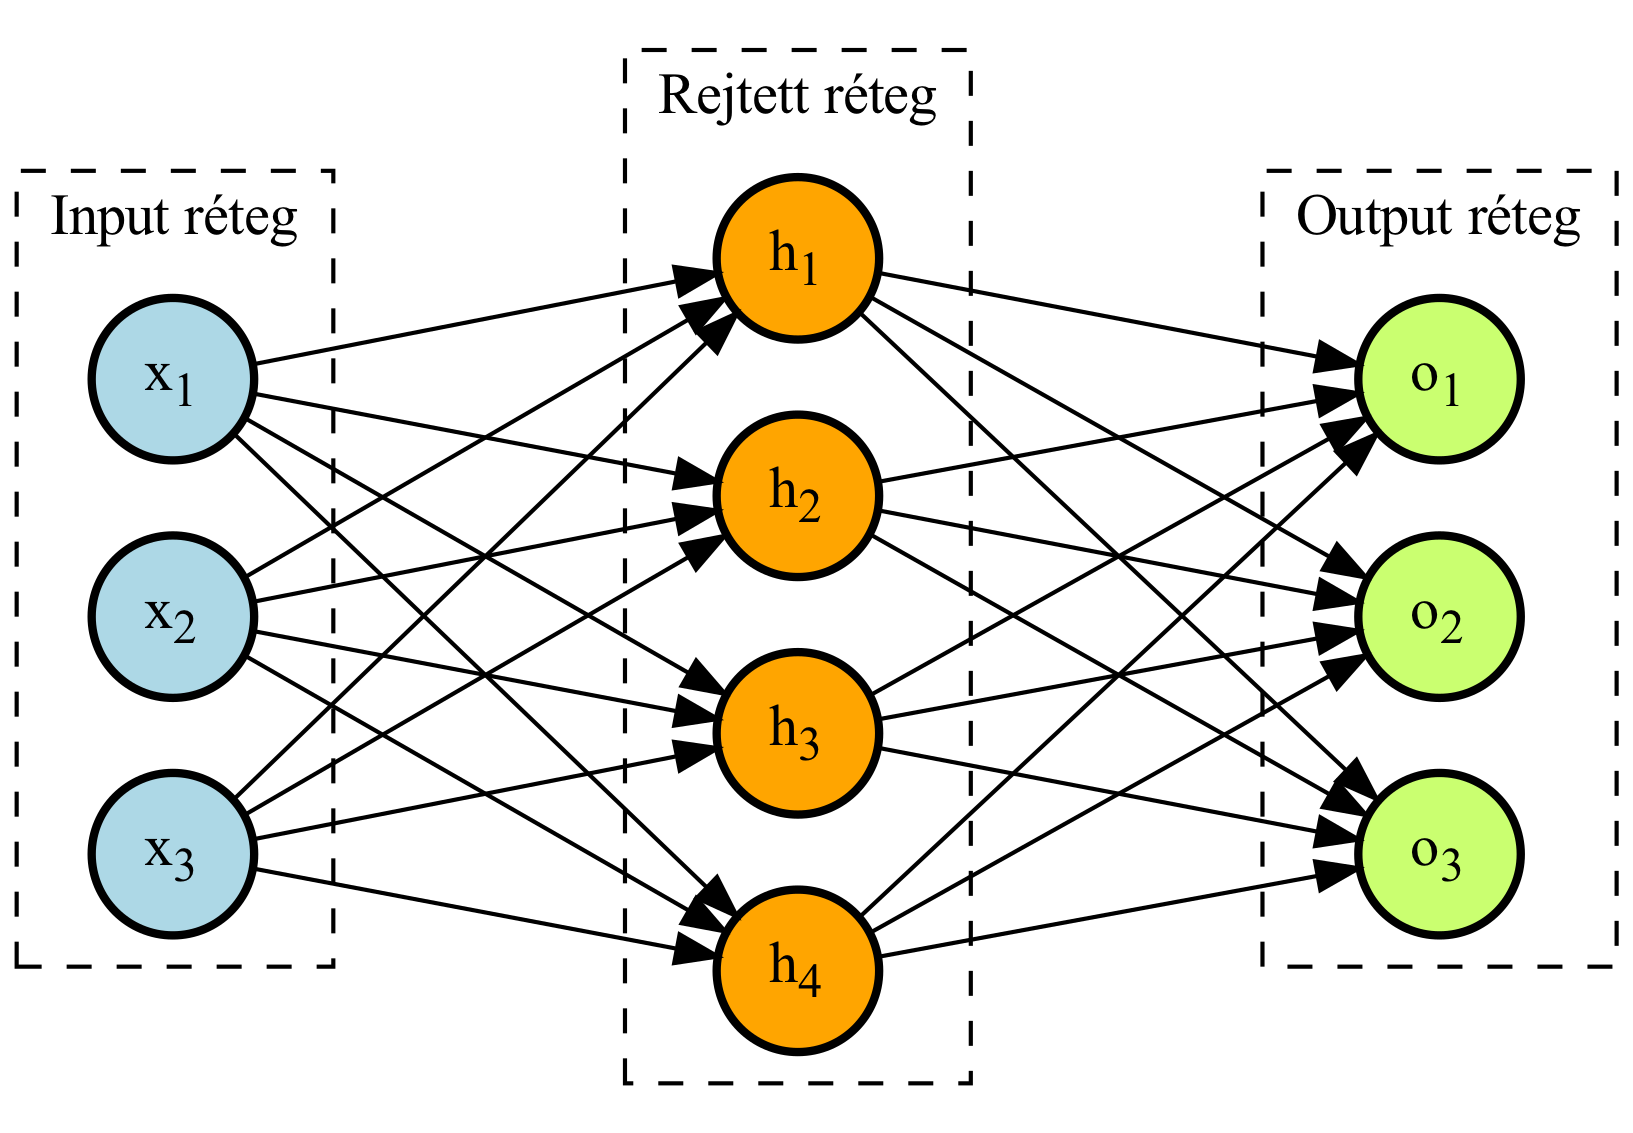
\includegraphics[width=7cm, height=7cm, keepaspectratio]{graphs/neural_9.png}
\end{center}
\end{column}
\end{columns}
\end{frame}

\section{Tanítás}

\begin{frame}
\tableofcontents[currentsection]
\end{frame}

\begin{frame}{A perceptron tanítása}
\begin{columns}
\begin{column}{.5\textwidth}
\only<1-3>{Tanítás során egyszerre egy mintaegyed áramlik át a hálózaton. \textbf{A modell a mintaegyedre predikciót készít, majd összeveti a címkével.} Ennek alapján tudja kiszámítani a költséget és frissíteni a súlyait.}
\only<4>{
\begin{block}{Perceptron tanítás szabálya}
\[
w_{i,j} \leftarrow w_{i,j} + \alpha	 \left( y_j - \hat{y}_j \right) x_i
\]
Ahol: 
\begin{itemize}
	\item $w_{i,j}$: Kapcsolati súly az $i$ input neuron és $j$ output neuron között
	\item $x_i$: Aktuális mintaegyed
	\item $\hat{y}_j$: $j$ output neuron predikciója
	\item $y_j$: $j$ neuronhoz tartozó címke
	\item $\alpha$: Tanulási sebesség
\end{itemize}
\end{block}}
\end{column}
\begin{column}{.5\textwidth}
\begin{center}
\includegraphics<1>[width=7cm, height=7cm, keepaspectratio]{images/neural_3.png}
\includegraphics<2>[width=7cm, height=7cm, keepaspectratio]{images/neural_4.png}
\includegraphics<3>[width=7cm, height=7cm, keepaspectratio]{images/neural_5.png}
\includegraphics<4>[width=7cm, height=7cm, keepaspectratio]{images/neural_6.png}
\end{center}
\end{column}
\end{columns}
\end{frame}

\begin{frame}{Neurális hálózat tanítása}
\begin{columns}
\begin{column}{.5\textwidth}
\only<1>{Egy teljes neurális hálót a perceptrontól különbözően kell tanítani, mert több egységből áll. Ennek eljárása a \textbf{hiba visszaterjesztő algoritmus}.\par\medskip
A hiba visszaterjesztő algoritmus összesen két iteráció alatt (egy előre, egy hátra) képes becslést adni a hálózat minden súlyára.\par\medskip
A mintaegyedek kötegekben áramlanak át a hálózaton. A kötegek mérete szabályozható. Minden köteg feldolgozása után kerül sor hiba számításra és visszaáramoltatásra.}
\only<2>{\begin{enumerate}
	\item Egy köteget átenged a hálózaton, és közben minden réteg predikcióját elmenti.
	\item Hálózat output hibájának kiszámítása
	\item Kiszámolja, hogy az egyes kimeneti kapcsolatok mennyiben járultak hozzá a teljes hibához. 
	\item Kiszámolja, hogy a kimeneti kapcsolatok hibái mennyiben származtathatók az előző kapcsolatok hibájából, majd ezt elvégzi minden rétegre. 
	\item Súlyok frissítése a hibáik alapján.
\end{enumerate}}
\end{column}
\begin{column}{.5\textwidth}
\begin{center}
\includegraphics<1>[width=7cm, height=7cm, keepaspectratio]{graphs/neural_10.png}
\includegraphics<2>[width=7cm, height=7cm, keepaspectratio]{graphs/neural_11.png}
\end{center}
\end{column}
\end{columns}
\end{frame}

\begin{frame}{Tanulási sebesség}
\begin{columns}
\begin{column}{.4\textwidth}
A frissítések mérete a tanulási sebességtől és az optimalizálótó algoritmusól függ. Az optimális tanulási sebességre az iterációnkénti költségből lehet következtetni.\par\medskip
\textbf{Érdemes először egy magasabb tanulási sebességgel elkezdeni a tanítást, majd folyamatosan csökkenteni. }
\end{column}
\begin{column}{.6\textwidth}
\begin{center}
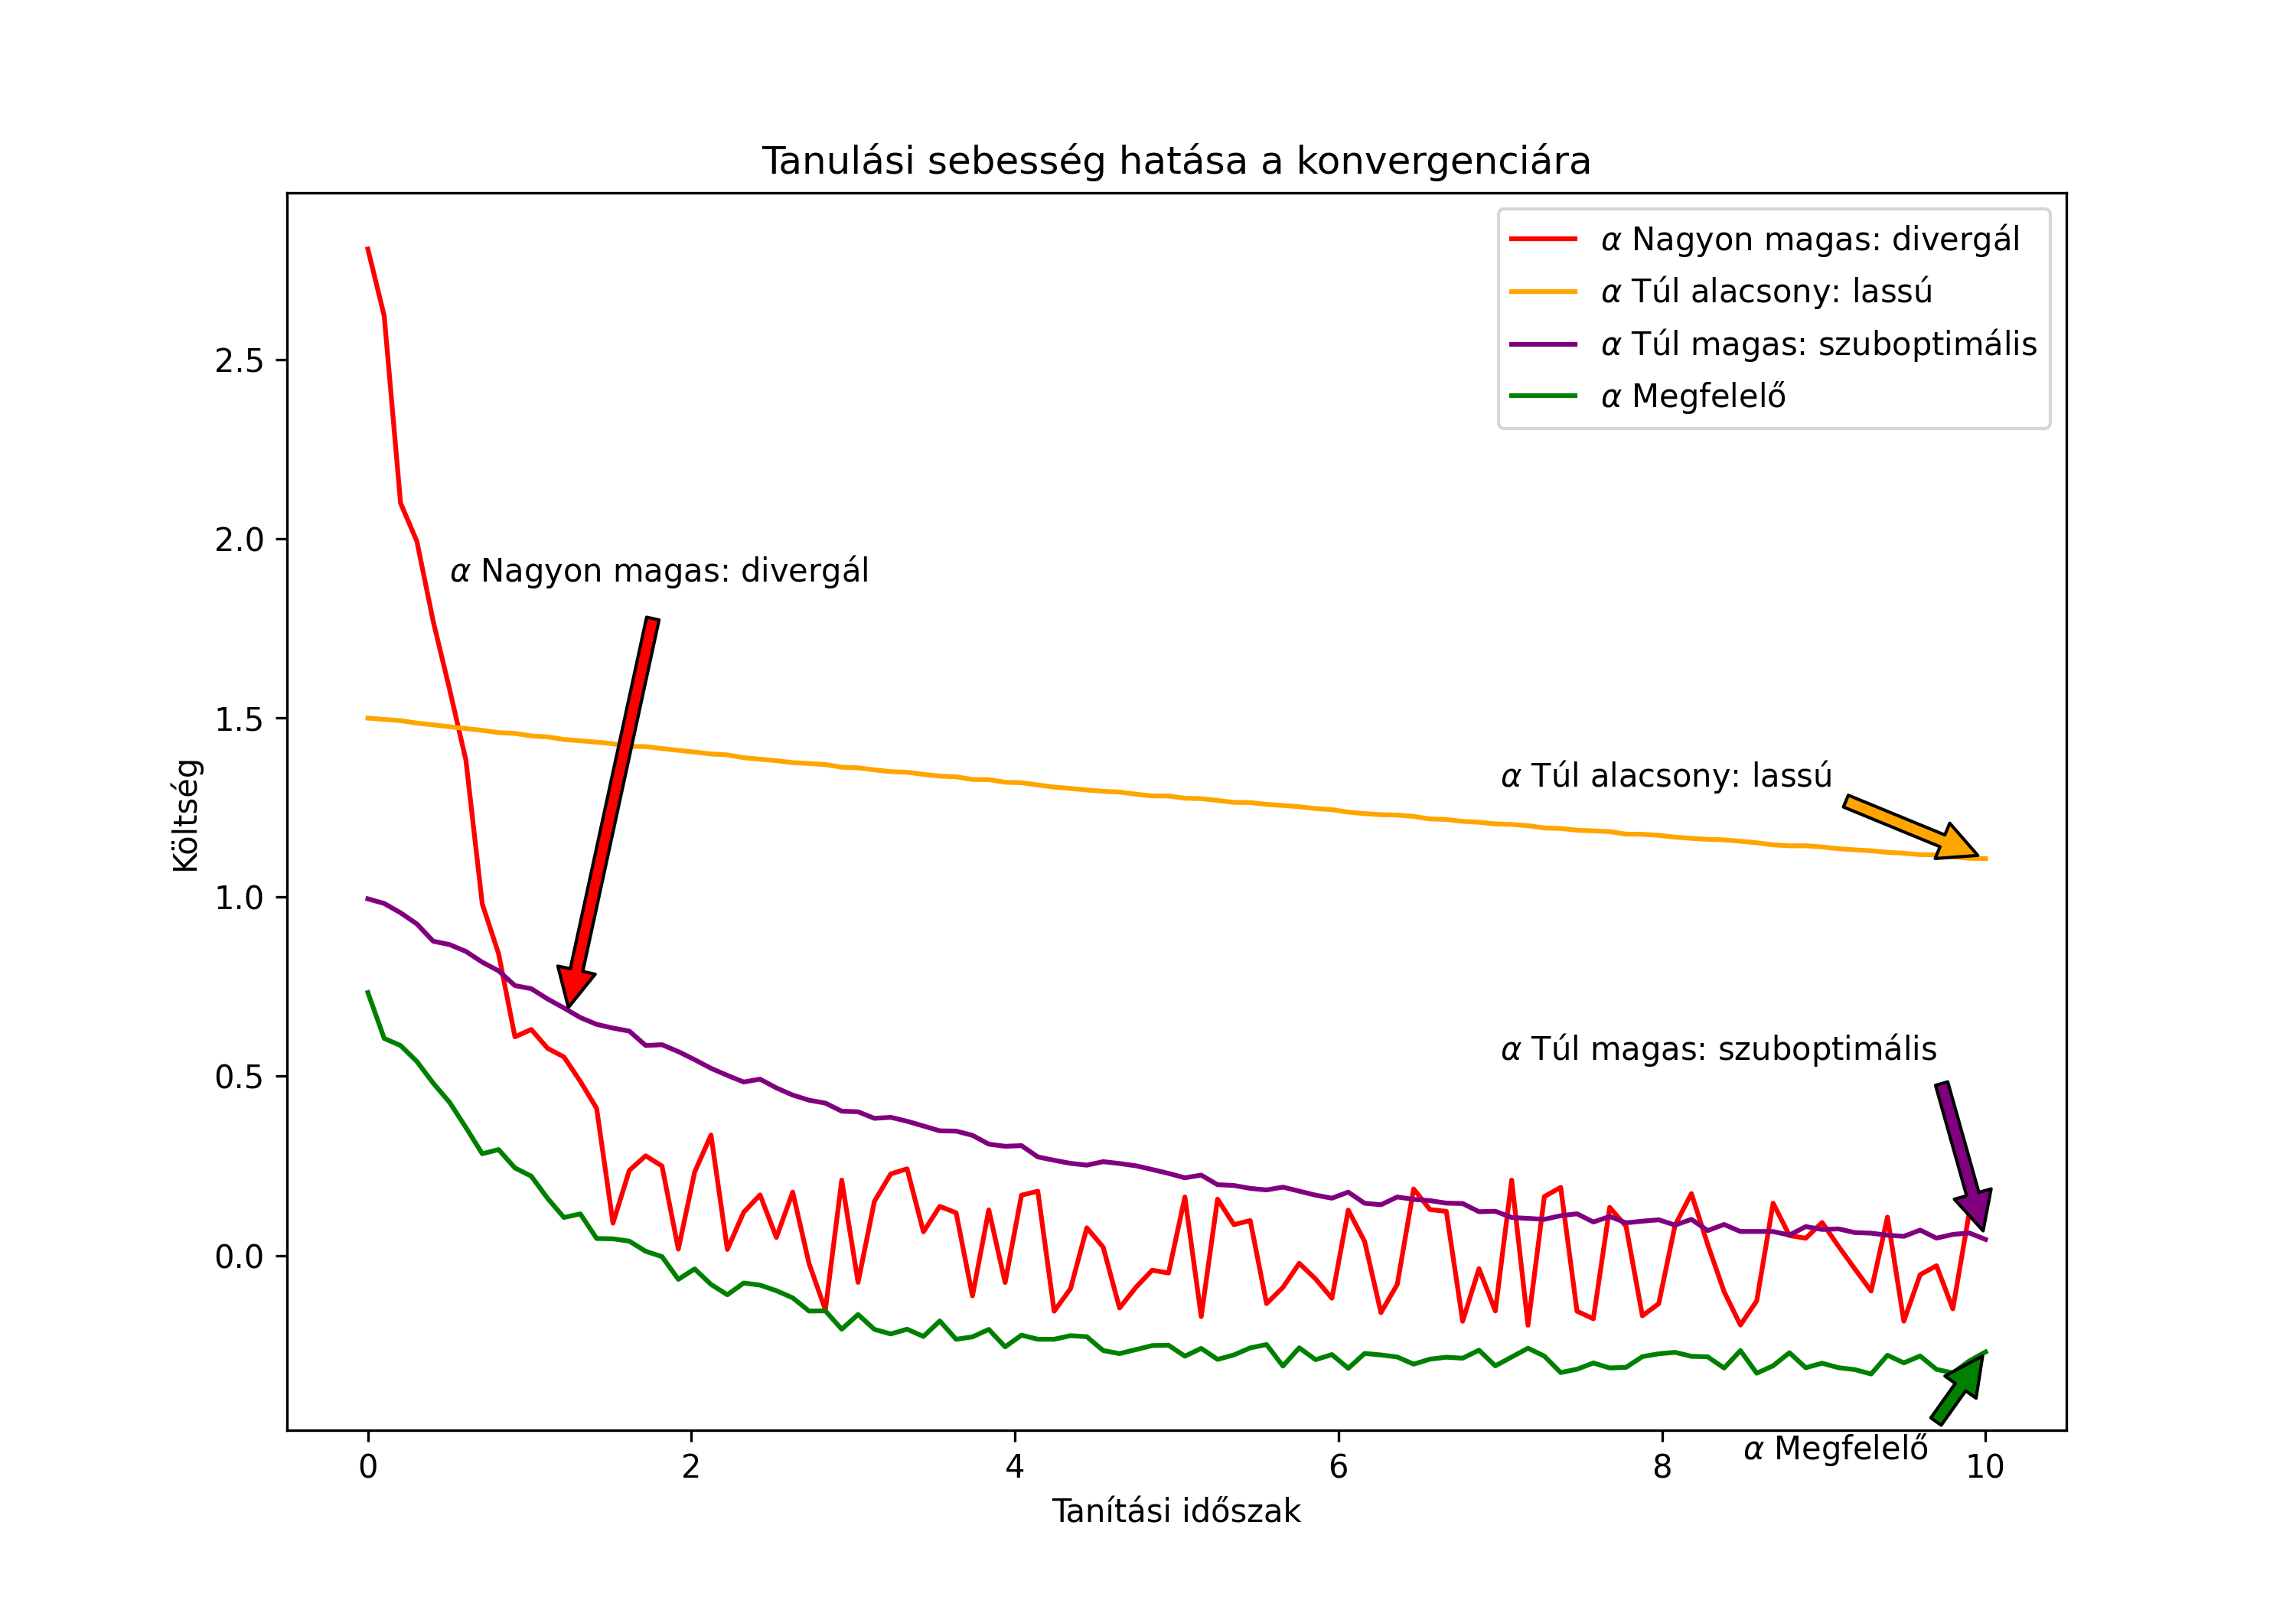
\includegraphics[width=9.5cm, height=7cm, keepaspectratio]{images/neural_7.png}
\end{center}
\end{column}
\end{columns}
\end{frame}

\begin{frame}{Regularizáció neurális hálók esetén}
\begin{columns}
\begin{column}{.5\textwidth}
\only<1>{\textbf{A neurális hálózatok fogékonyak a túltanulásra, ha túlságosan magas a paraméterek száma.}\par\medskip
Az optimalizálás során lehetséges az $\ell_1, \ell_2$ normák használata, ez nagyon hasonló működést fog eredményezni, mint a LASSO vagy Ridge regressziók esetén.}
\only<2>{Egy másik regularizációs eljárás a \textbf{kiesés}. \textbf{Kiesés során minden neuron kap $p$ valószínűséget arra, hogy ne legyen figyelembe véve a tanítás során.} Ez általában 50\%.\par\medskip
Kieséssel minden tanítási lépésben egy egyedi architektúra tanul, ez összesen $2^N$ lehetőség.}
\end{column}
\begin{column}{.5\textwidth}
\begin{center}
\includegraphics<1>[width=7cm, height=7cm, keepaspectratio]{graphs/neural_10.png}
\includegraphics<2>[width=7cm, height=7cm, keepaspectratio]{graphs/neural_12.png}
\end{center}
\end{column}
\end{columns}
\end{frame}

\begin{frame}{Transzfertanulás}
\begin{columns}
\begin{column}{.5\textwidth}
Általában nem célszerű egy komplex mélyhálózatot a semmiből feltanítani.\par\smallskip
\textbf{Egy jobb megoldás egy hasonló feladatot ellátó neurális hálózat súlyainak átemelése az újonnan létrehozott modellbe.}\par\smallskip
Minél hasonlóbbak a feladatok, annál több réteget lehet felhasználni a már meglévő hálózatból.
\end{column}
\begin{column}{.5\textwidth}
\begin{center}
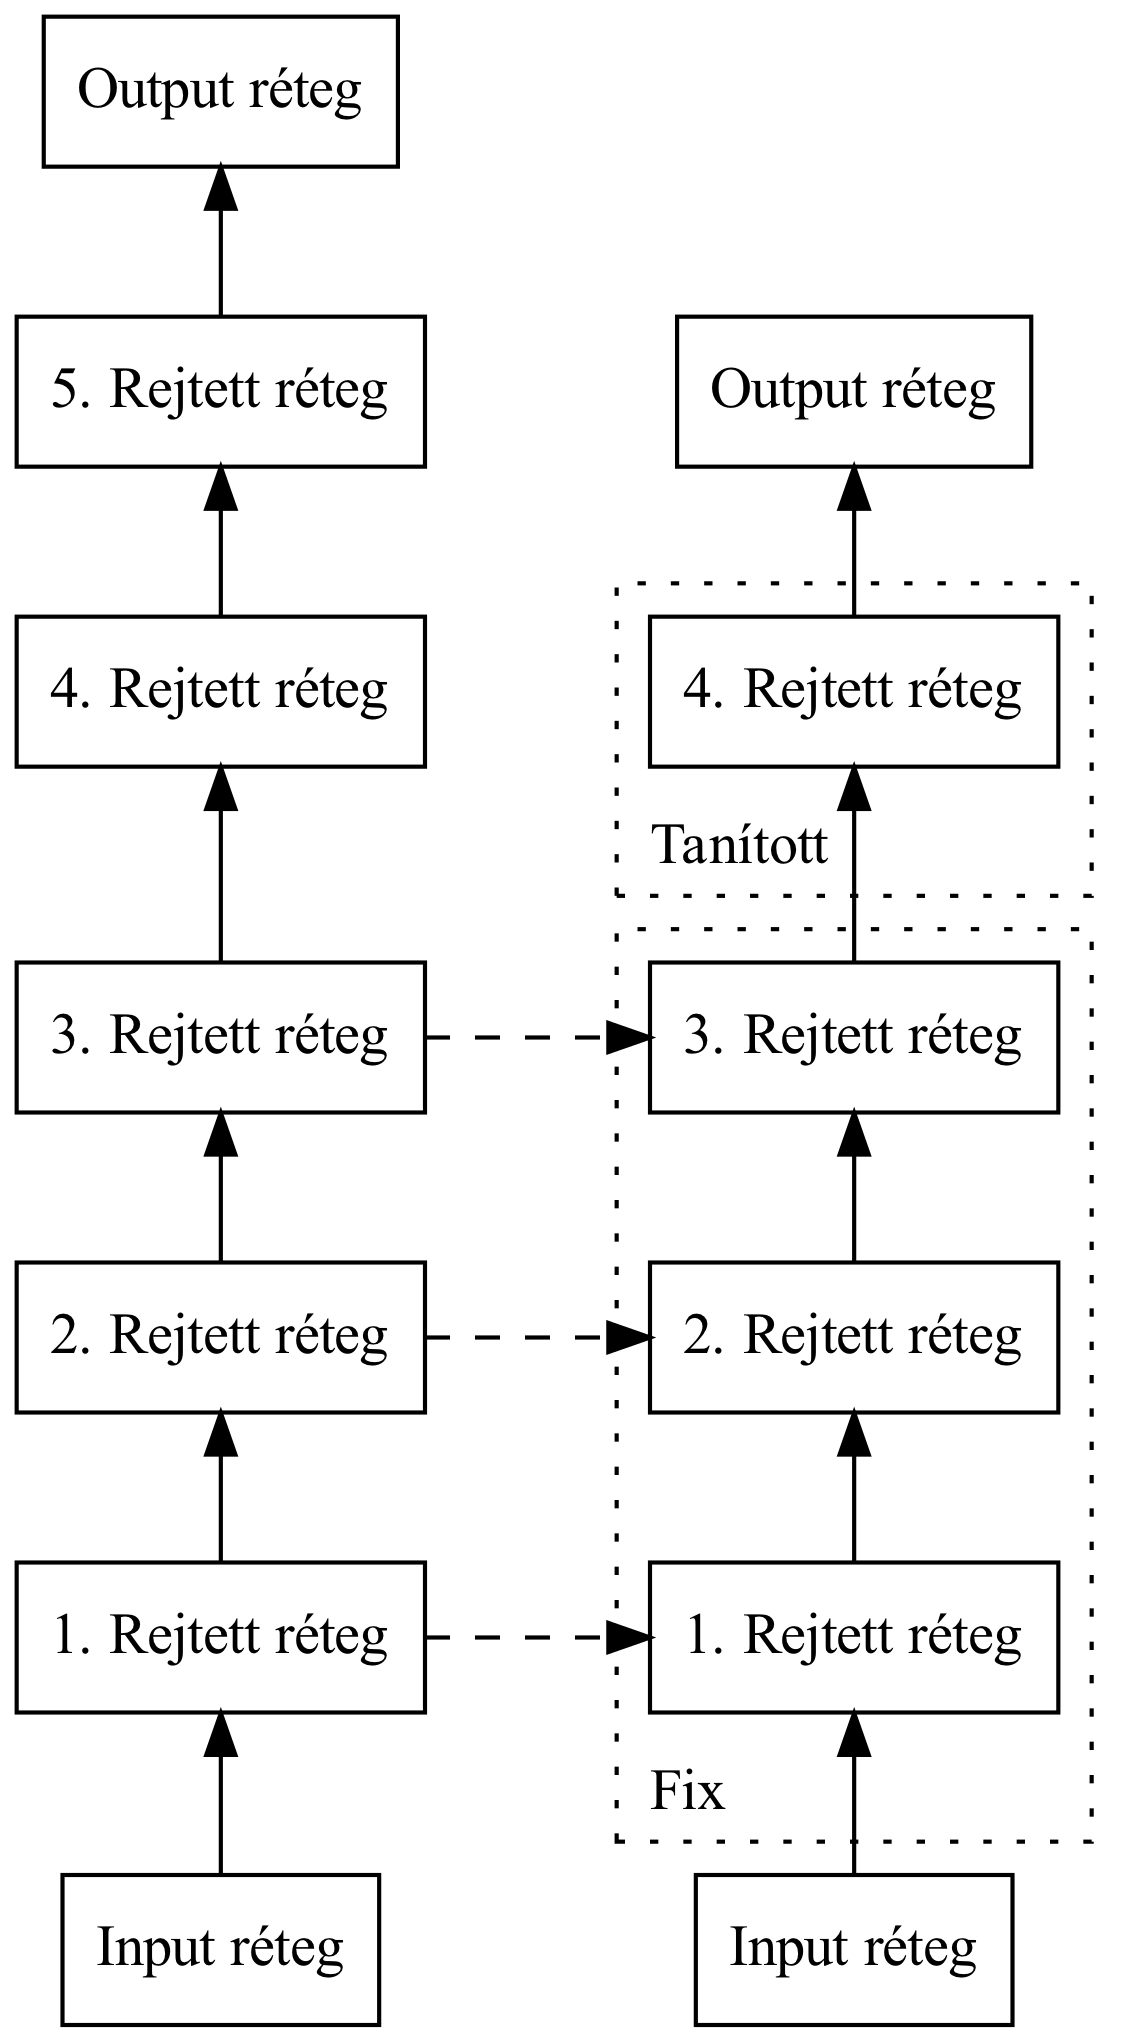
\includegraphics[width=7cm, height=7cm, keepaspectratio]{graphs/neural_13.png}
\end{center}
\end{column}
\end{columns}
\end{frame}

\section{Konvolúciós hálózatok}

\begin{frame}
\tableofcontents[currentsection]
\end{frame}

\begin{frame}{A biológiai látás alapjai}
David H. Hubel és Torsten Wiesel macskákon mutatták meg, hogy \textbf{a látókéregben a neuronoknak befogadó mezője van}, azaz csak a vizuális térnek egy bizonyos szegmensén elhelyezett ingerületet képesek befogadni.\par\smallskip
Vannak olyanok, amelyek csak vertikális, vagy horizontális alakokat érzékelnek. \textbf{A neuronok különböző befogadó mezői átfedésben állhatnak egymással, és együtt alakítják ki a vizuális teret.}\par\smallskip
\begin{center}
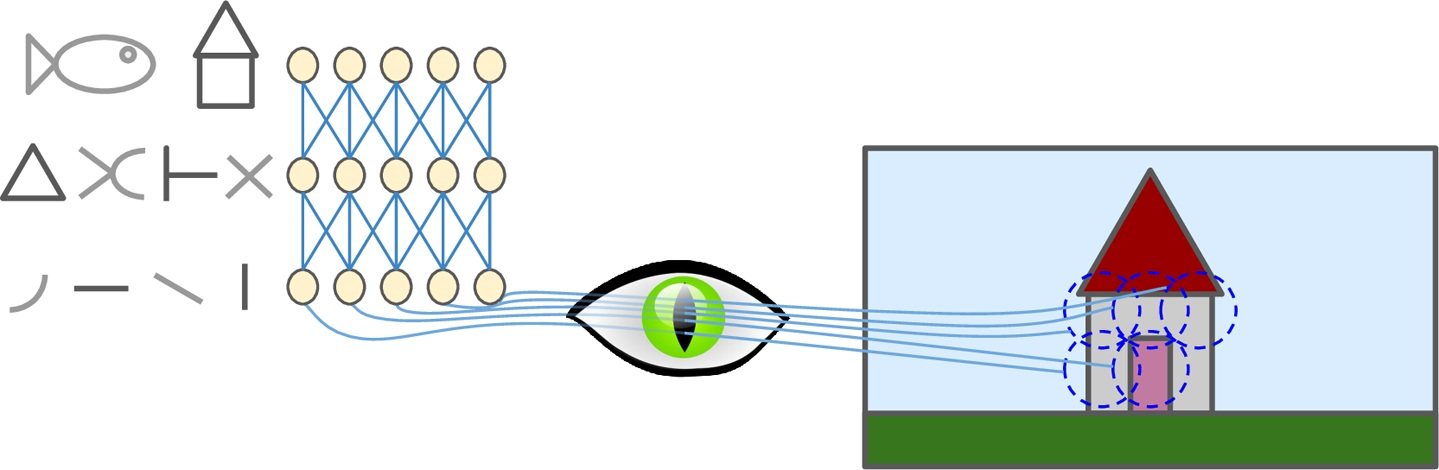
\includegraphics[width=11cm, height=7cm, keepaspectratio]{images/neural_8.png}
\end{center}
\end{frame}

\begin{frame}{Konvolúciós hálózati architektúra}
A konvolúciós hálókban a \textbf{konvolúciós és pooling rétegek felelnek a képi jellemzők alacsony szintű feldolgozásáért}. Ezután teljesen becsatolt rétegek következnek. Az output réteg felépítése megegyezik a korábban definiáltakkal.\par\smallskip
\begin{center}
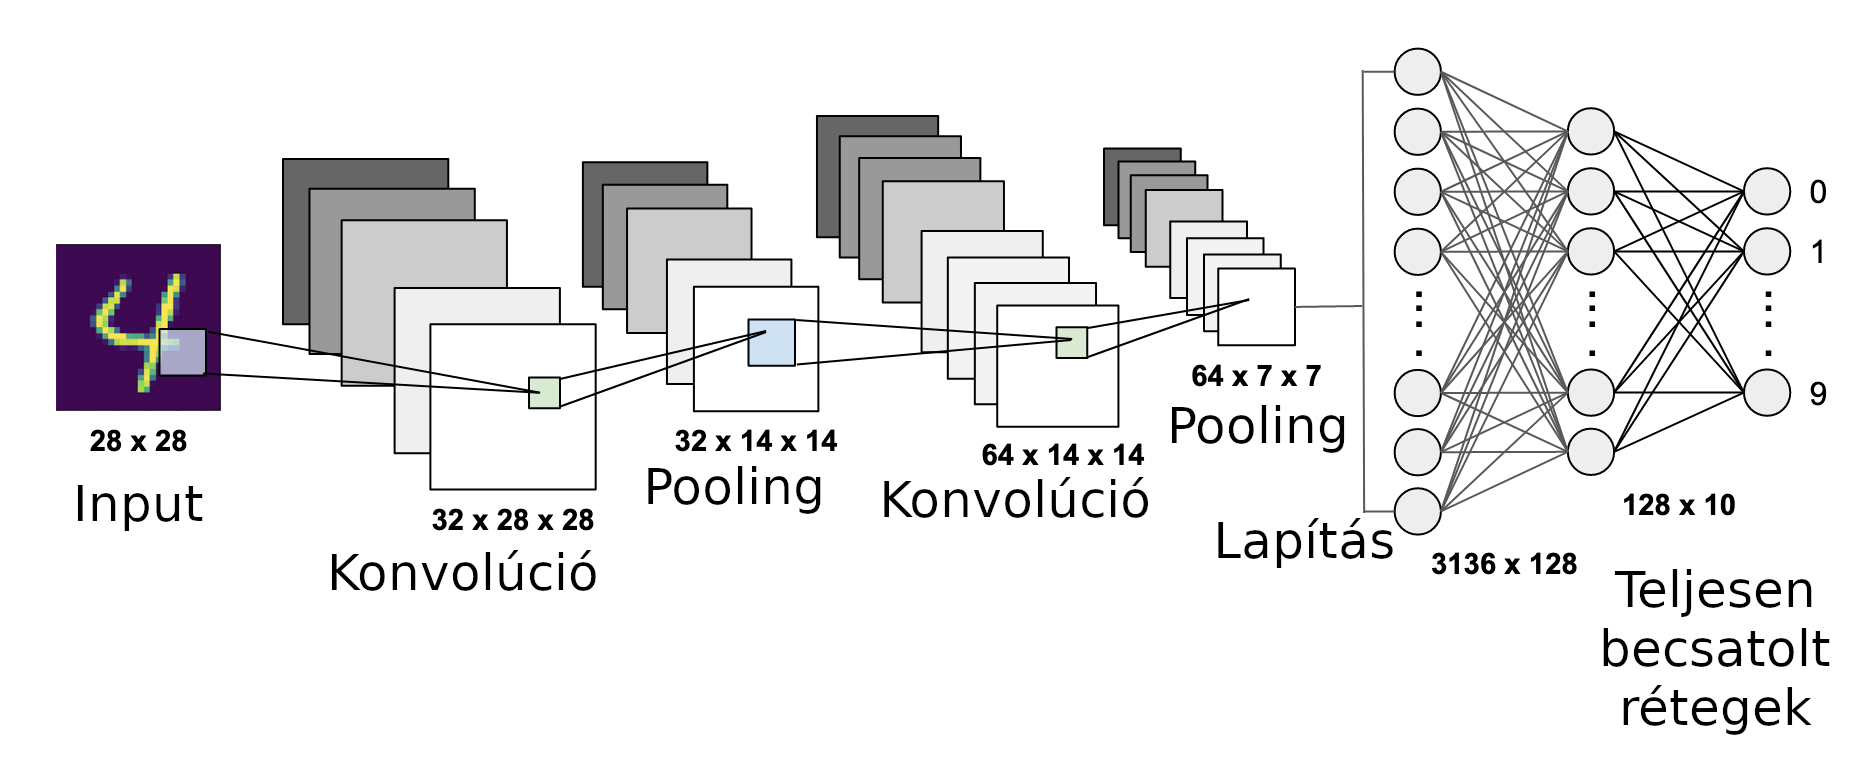
\includegraphics[width=12cm, height=7cm, keepaspectratio]{images/neural_9.png}
\end{center}
\end{frame}

\begin{frame}{A konvolúció művelete}
\begin{columns}
\begin{column}{.6\textwidth}
A konvolúció egy matematikai művelet, ami két függvényt kombinál egy harmadikká. Egy \textbf{jelfüggvényt} valamilyen \textbf{magfüggvénnyel} vegyít egy outputtá, ami megadja, hogy \textbf{a mag mennyiben befolyásolja a jelet}. 
\begin{block}{Konvolúció (2D, diszkrét)}
A diszkrét konvolúció két 2D függvényen értelmezett, és jellemzők kivonatolására, szűrők alkalmazására használatos. Konvolúció $f$ jel- és $g$ magfüggvényen, $i,j$ képkoordinátákra:
\[
(f \textasteriskcentered g)[i, j] = \sum_{m=-\infty}^\infty \sum_{n=-\infty}^\infty g[i-m, j-n]f[m,n]
\]
\end{block}
\end{column}
\begin{column}{.4\textwidth}
\begin{center}
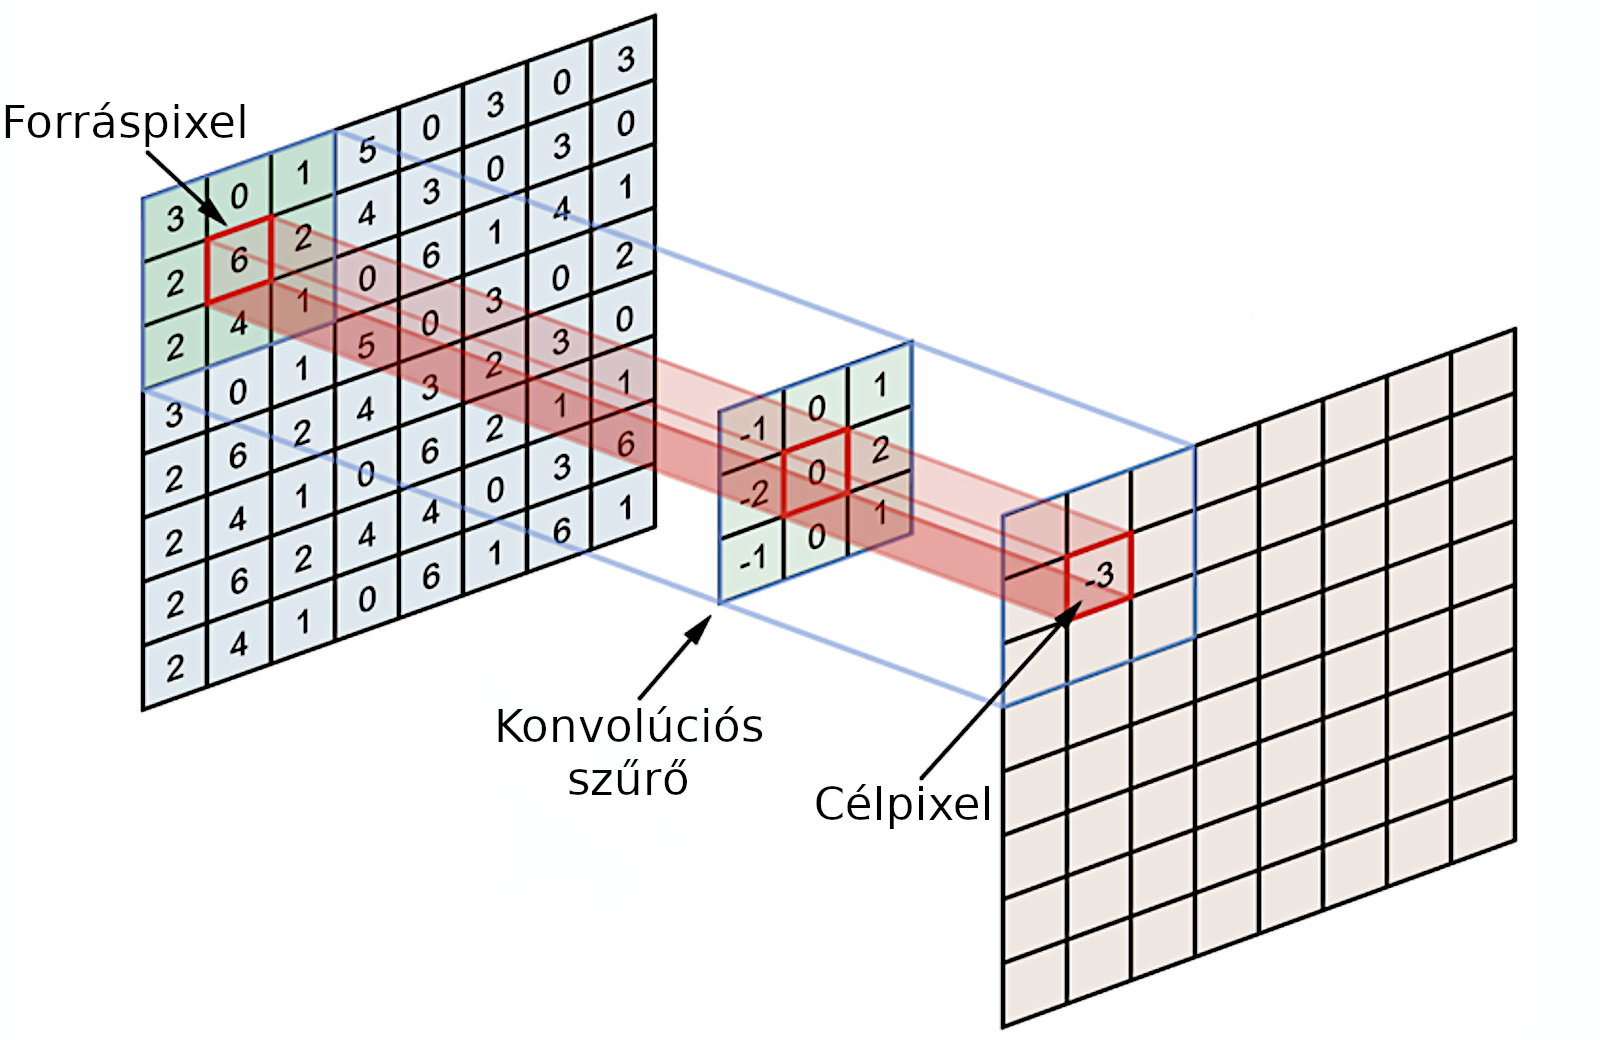
\includegraphics[height=6cm, width=6cm, keepaspectratio]{images/neural_10.png}
\end{center}
$(-1 \cdot 3) + (0 \cdot 0) + (1 \cdot 1) +$\\
$(-2 \cdot 2) + (0 \cdot 6) + (2 \cdot 2) +$\\
$(-1 \cdot 2) + (0 \cdot 4) + (1 \cdot 1) = -3$\\
\end{column}
\end{columns}
\end{frame}

\begin{frame}{Konvolúciós rétegek}
\begin{columns}
\begin{column}{.5\textwidth}
A neurális hálózatok konvolúciós rétegeiben a \textbf{tanítható súlyok az egyes forráspixelekhez tartozó konvolúciós szűrőkben elhelyezkedő értékek}. Ez minden forráspixelhez egy egyedi szűrőt jelent, de lehetséges tetszőleges számú szűrő is.\par\smallskip
Ez az architektúra lehetővé teszi alacsony szintű jellemzők leképezését a mélyrétegekben, és a magas szintűek leképezését a sekély rétegekben.
\end{column}
\begin{column}{.5\textwidth}
\begin{center}
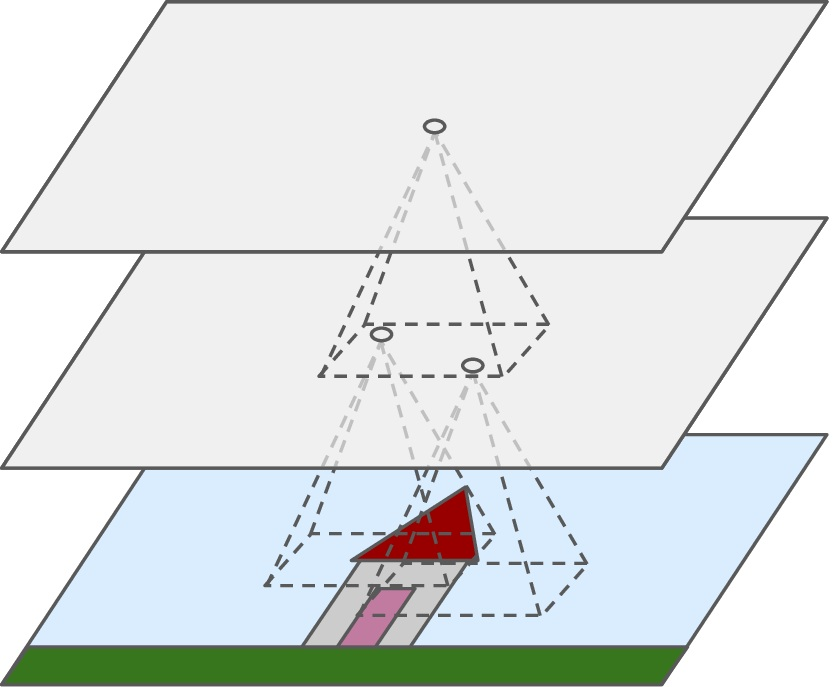
\includegraphics[width=6cm, height=7cm, keepaspectratio]{images/neural_11.png}
\end{center}
\end{column}
\end{columns}
\end{frame}

\begin{frame}{Konvolúciós neuronok kapcsolatai}
\begin{columns}
\begin{column}{.5\textwidth}
\only<1>{Ha adott egy $f_h \cdot f_w$ szélességű konvolúciós szűrő az $i,j$ pozíción és $s$ lépésmérettel, ennek a befogadó mezőjének a szélessége:
\begin{block}{}
\vspace{-.2cm}
\[
rf_w = f_w + \left( i-1 \right) \cdot \left( s-1 \right)
\]
\end{block}
és magassága:
\begin{block}{}
\vspace{-.2cm}
\[
rf_h = f_h + \left( j-1 \right) \cdot \left( s-1 \right)
\]
\end{block}}
\only<2>{\begin{block}{Zero-padding}
Az input kép körbevétele $0$ értékekkel, hogy elkerülhető legyen a konvolúciós műveletből adódó méretcsökkenés.
\end{block}}
\only<3>{\begin{block}{Lépésméret}
A konvolúciós szűrők lépésmérete az $x$ tengely mentén $s_w$, az $y$ tengely mentén $s_h$ azt szabályozza, hogy a konvolúciós kernel (szűrő) milyen mértékben mozog át az input kép pixelein a konvolúció során.\par\smallskip
Nagyobb lépésméret kisebb jellemzőméretet eredményez.
\end{block}}
\end{column}
\begin{column}{.5\textwidth}
\begin{center}
\includegraphics<1-2>[width=7cm, height=7cm, keepaspectratio]{images/neural_12.png}
\includegraphics<3>[width=7cm, height=7cm, keepaspectratio]{images/neural_13.png}
\end{center}
\end{column}
\end{columns}
\end{frame}

\begin{frame}{Konvolúciós szűrők}
\begin{columns}
\begin{column}{.5\textwidth}
\only<1>{A konvolúciós neuron súlyai reprezentálhatók egy konvolúciós szűrővel. A neuron ezeket a súlyokat finomhangolja a céltól függően.}
\only<2->{Az ábrákon vertikális, majd horizontális szűrővel konvolvált képek láthatók. A szűrők egy tengelyen $1$ értéket vesznek fel, mindenhol máshol $0$ értékeket.}
\begin{center}
\includegraphics<2>[width=7cm, height=3.5cm, keepaspectratio]{images/neural_15.png}
\includegraphics<3>[width=7cm, height=3.5cm, keepaspectratio]{images/neural_17.png}
\end{center}
\end{column}
\begin{column}{.5\textwidth}
\begin{center}
\includegraphics<1>[width=7cm, height=7cm, keepaspectratio]{images/neural_14.png}
\includegraphics<2>[width=7cm, height=7cm, keepaspectratio]{images/neural_16.png}
\includegraphics<3>[width=7cm, height=7cm, keepaspectratio]{images/neural_18.png}
\end{center}
\end{column}
\end{columns}
\end{frame}

\begin{frame}{A lazító (pooling) réteg}
\begin{columns}
\begin{column}{.5\textwidth}
A lazító rétegek feladata, hogy almintázzák a bemeneti jellemzőket annak érdekében, hogy kisebb legyen a memóriaigény és a paraméterek száma.\par\medskip
\textbf{A lazító neuron aggregálja a kapcsolatai által elérhető neuronok értékeit.} Az aggregáló művelet lehet például $max$, $avg$ stb...
\end{column}
\begin{column}{.5\textwidth}
\begin{center}
\includegraphics<1>[width=7cm, height=7cm, keepaspectratio]{images/neural_19.png}
\includegraphics<2>[width=7cm, height=7cm, keepaspectratio]{images/neural_20.png}
\includegraphics<3>[width=7cm, height=7cm, keepaspectratio]{images/neural_21.png}
\includegraphics<4>[width=7cm, height=7cm, keepaspectratio]{images/neural_22.png}
\includegraphics<5>[width=7cm, height=7cm, keepaspectratio]{images/neural_23.png}
\end{center}
\end{column}
\end{columns}
\end{frame}

\begin{frame}{Lazítás a gyakorlatban}
\begin{columns}
\begin{column}{.5\textwidth}
\textbf{A memória- és paraméterszám csökkentése mellett a lazítás művelete bevezet egy alacsony fokú invarianciát kisebb eltolásokkal szemben}.\par\smallskip
Érdemes megfigyelni, hogy az $A$ és $B$ képek esetén a pooling ugyanazt az outputot eredményezte, viszont ahogy az input kép jobban eltolódik, az output is megváltozik.
\end{column}
\begin{column}{.5\textwidth}
\begin{center}
\includegraphics<1>[width=7cm, height=7cm, keepaspectratio]{images/neural_24.png}
\includegraphics<2>[width=7cm, height=7cm, keepaspectratio]{images/neural_25.png}
\includegraphics<3>[width=7cm, height=7cm, keepaspectratio]{images/neural_26.png}
\end{center}
\end{column}
\end{columns}
\end{frame}

\begin{frame}{Adataugmentáció}
\begin{columns}
\begin{column}{.5\textwidth}
Új tanító egyedek létrehozása a meglévőkön végzett változtatások segítségével mint:
\begin{itemize}
	\item Forgatás
	\item Eltolás
	\item Sötétítés
	\item Közelítés
	\item Távolítás
	\item Világosítás
\end{itemize}
\end{column}
\begin{column}{.5\textwidth}
\begin{center}
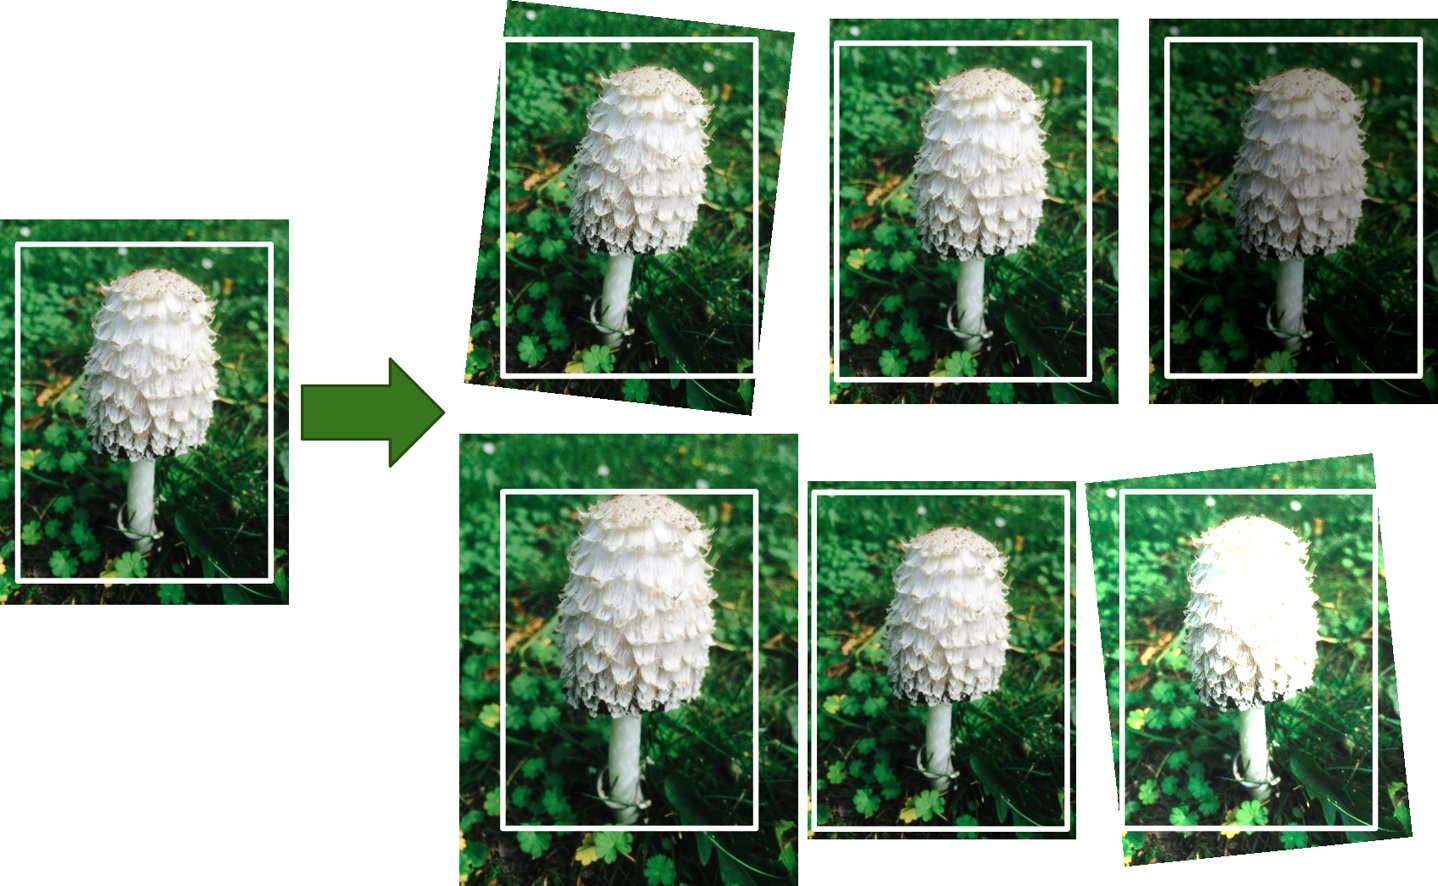
\includegraphics[width=7cm, height=7cm, keepaspectratio]{images/neural_27.png}
\end{center}
\end{column}
\end{columns}
\end{frame}

\end{document}























